\section{Android  を標的にしたマルウェア}
本研究では,Android を標的にしたマルウェアの中で,悪意ある Android アプリケーションを対象とする.
\ref{sec:malware}節では,悪意あるアプリケーションの挙動と,不正な振る舞いをするために何をしているのかについて説明する.
また,マルウェアの例の 1 つとして,GoldDream の挙動を説明する.
\ref{sec:andrapp}節では,基本的な Android アプリケーションの構成について説明する.
Android アプリケーションの概要を示している AndroidManifest.xml とアプリケーションの実行ファイルである,classes.dex,そして画像ファイルが入っているディレクトリについて説明する.

\subsection{悪意ある Android アプリケーション}
\label{sec:malware}
マルウェアの主な挙動として,個人情報の盗難と不正な金銭請求がある.
個人情報に関して言えば,デスクトップ PC やノートパソコンに比べ,スマートフォンは,電話帳,メールなど個人情報のデータの量が多いため,攻撃者の標的になりやすいのは明らかである.
スマートフォンでもネットサービス等で銀行口座の操作ができるため,スマートフォンのブラウザに銀行アカウントのパスワードが残っている可能性もある.
もし銀行アカウントのパスワードが盗まれた場合,多額の被害を生んでしまうおそれがある.
ユーザ自身の情報だけでなく,端末の情報,つまり IMEI (端末識別番号),SIM カードの情報, GPS の位置情報なども盗まれている.
金銭を不正に請求するための攻撃方法として,SMS を使ったものがある.
SMS を使った攻撃の様子を 図\ref{SmsAttack}に示す.
SMS Premium Service は,ある番号へ SMS を送ることで音楽や動画などのコンテンツを買うことができるサービスである.
この攻撃は Premium Service のように,マルウェアが攻撃者たちの番号へ SMS を送信することで,ユーザーに課金させる方法だ,
その課金は携帯電話の料金の支払いと同時に行われ,そこで支払われた料金の一部が攻撃者たちに支払われる.
ユーザはその支払い請求が来るまで SMS が送られたことに気づかない.
通常の Premium Service ではユーザに支払い確認のメッセージがくるのだが,マルウェアはこれをブロックするためだ.

\begin{figure}[t]
\begin{center}
\graphicspath{{./epsfiles/}}
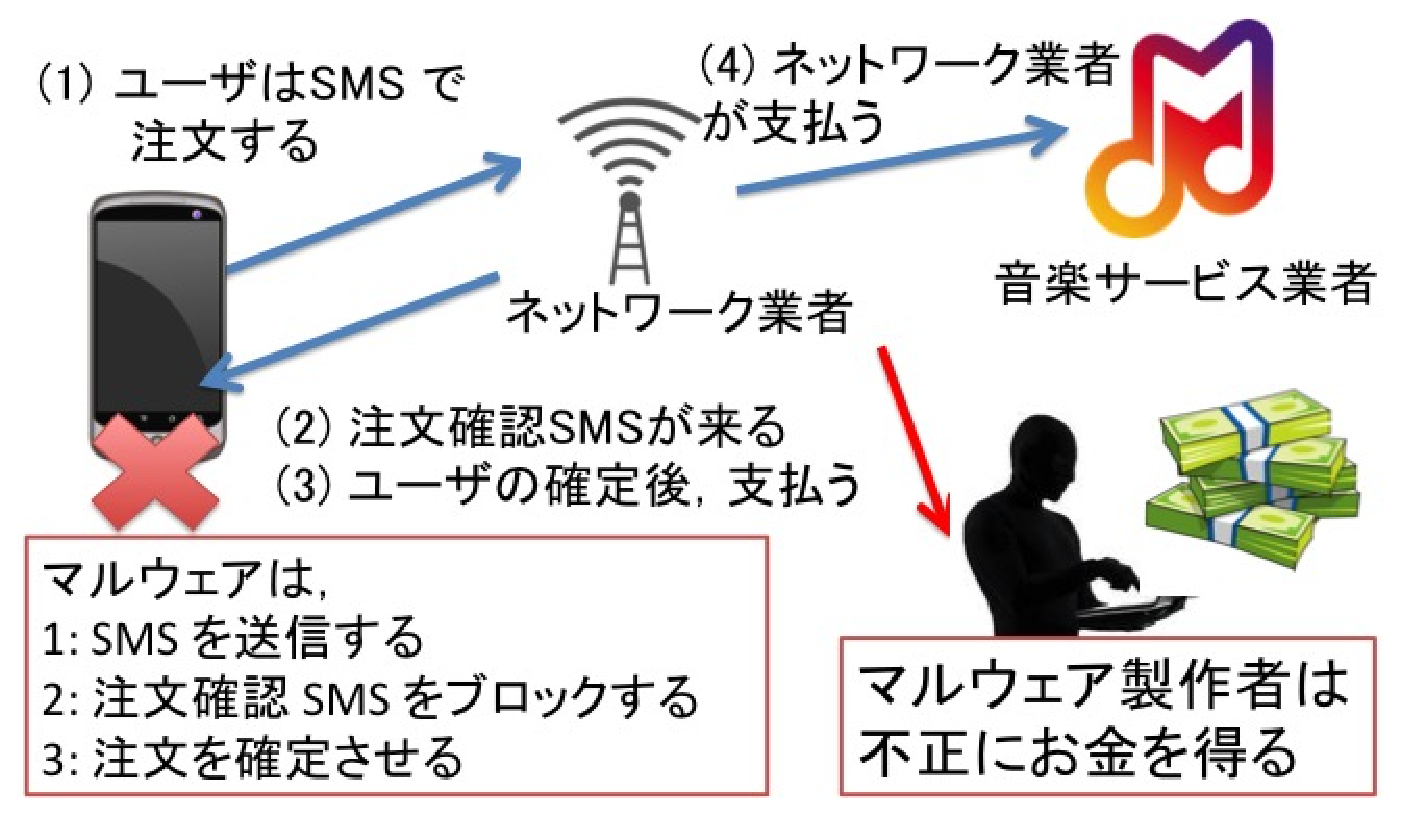
\includegraphics[ scale = 0.4]{sms3.eps}
\end{center}
\caption{SMS を使った攻撃}
\label{SmsAttack}
\end{figure}

マルウェアが先に述べたような攻撃をするための方法を 2 つ挙げる.
1 つは,外部からの遠隔操作だ\cite{remotectrl}.
マルウェアは外部サーバからの命令を受け取り,実行する.
あるマルウェアがインストールされると,外部のサーバから暗号化されたスクリプトを受け取り,そのスクリプトを復号化し,実行するという例もある.
この手法を使うと,マルウェアを検知するソフトウェアを回避することができる.
なぜなら,公式アプリケーションストア (Google Play)  にアップロードされた時点では不正な動きをするコードをマルウェア自身は何も持っていないために,このソフトウェアに検知されないからだ.
外部から得たスクリプトは DexClassLoader というクラスローダによりアプリケーションに読み込むことができる.
もう一つは,Android OS の脆弱性をつくことで,特権レベルを上げることである.
不正にマルウェア自身の特権レベルを上げるマルウェアの中には root 権限を奪うものもある.
マルウェアに root 権限を奪われてしまうと,ユーザが抵抗できる余地は少ないため,悪用されると非常に危険である.
マルウェアの 1 つである,AndroidDefender\cite{sopho}は,表向きにはウイルス対策アプリケーションとなっている.
AndroidDefender が起動すると,それは感染した端末から電話をかけられなくしたり,さまざまなアプリケーションへのアクセスを制限させる.
その後,AndroidDefender は端末を修復するためにユーザに大金を要求する.
 
実際のマルウェアの例として,GoldDream を紹介する.
GoldDream は端末情報を流出させるために,電話の発着信などのイベントを監視し,外部へと送信する.
そこで,GoldDream の挙動について説明する.
GoldDream はSMS の受信,電話の発着信があると,バックグラウンドでユーザに気づかれることなく起動される.
GoldDream はレシーバを登録することで,これらの着信が来た時に Android OS が出す通知を受け取れるようにしている.SMS を受信した際は,受信したメッセージの送り元のアドレス,内容,タイムスタンプを収集する.
電話の発着信の場合も同様に,電話番号やタイムスタンプといった情報が GoldDream によって集められる.
このような情報を利用することで,マルウェアは他の端末へ攻撃範囲を拡大することができる.
例えば,他の端末の情報を得ることができれば,感染した端末から他端末へマルウェアのダウンロードリンクを載せたメッセージなどを送ることができる.
これらの情報は一度ローカルファイルに保存された後,外部のサーバへ送信される.
GoldDream は外部サーバからコマンドを受け取り,実行する.
サーバから受け取るコマンドは,次の 4 つである.
1) SMS をバックグラウンドで送信する,2) 電話を発信する,3) アプリケーションをインストール,アンインストールする,4) ファイルをサーバへアップロードする. 
ファイルをアップロードするコマンドは端末の情報を送信するために用いられる.



\subsection{Android アプリケーションの構成}
\label{sec:andrapp}
1 つの Android アプリケーションは 1 つの APK ファイル (.apk) となってまとめられている.
Androidのアプリケーションを実行するためには,異なる種類の複数のファイルが必要である.
例えば,AndroidManifest.xml, 画像ファイル,レイアウトファイル(png, jpg, xml, etc),classes.dex, アプリケーションの証明書である.
これらを1 つのファイルに ZIP 形式でまとめたものが APK ファイルである.
そのため,zip ファイルと同様に解凍,圧縮,中身の入れ替えができる.
よって,unzip コマンド で APK ファイルを解凍することができる.
APK ファイルを解凍すると,AndroidManifest.xml, classes.dex, res ディレクトリ,META-INF ディレクトリが展開される.
res ディレクトリには,アプリケーションのアイコン画像,アプリケーション実行時に画面上に表示する画像ファイルが入っている.
META-INF ディレクトリにはアプリケーションの証明書のファイルがある.
ただし,unzip コマンドで解凍した場合,AndroidManifest.xml はバイナリのままであるため,このファイルの中身を見たい場合は,apktool\cite{apktool}というツールを使う必要がある.
これらのファイルを一つの APK ファイルにまとめるのは,他のアプリケーションも同じファイル名を用いているためだ.
どのアプリケーションも必ず AndroidManifest.xml と classes.dex の 2 つのファイルを持っている.
そのため,これらのファイルはアプリケーションごとにまとめて端末上にインストールされる必要性がある.
そうすることで,Android OS はアプリケーションを管理することができる.

AndroidManifest.xml とはアプリケーションの基本的な情報が書かれている XML 形式のファイルである.
あるゲームアプリケーションの AndroidManifst.xml の例を図\ref{manif}に示す.
アプリケーションのパッケージ名,アプリケーションが使用する権限,アプリケーションが起動した時に最初に実行されるクラスなどが記されている.
パッケージ名は OS がアプリケーションを識別する名前である.
図\ref{manif}の 2 行目に.このアプリケーションのパッケージ名 (com.gamelio.DrawSlasher) が書いてある.
パッケージ名は待ち受け画面でアイコンの下に表示される名前とは異なる.
例えば,Facebook,Instagram の Android アプリケーションの場合はそれぞれ,com.facebook.katana,com.instagram.android となっている.
一般的にアプリケーションを使用している分には,ユーザはパッケージ名について気にする必要がないので,Android 端末を使用していてアプリケーションのパッケージ名を目にすることはまずない.
ただし,Android Debug Bridge (adb) を用いてターミナルからアプリケーションを手動でアンインストールする場合は,パッケージ名を特定する必要がある.
OS monitor という Android のシステム状況を確認できるアプリケーションを使うと,AndroidManifest.xml を見なくても,実行中のアプリケーションのパッケージ名を端末上で見ることができる.

Androidのアプリケーションは OS から権限を得ないと実行できないことがいくつもある.
たとえば電話の着発信,SMS の送受信, インターネットへの接続などである.
AndroidManifest.xml にこれらの権限を記すことにより,アプリケーションはその権限を得る.
これらの機能をアプリケーションで実行するためには,必ず AndroidManifest.xml に宣言しないといけない.
図\ref{manif}の中では,24 行目から38 行目にかけてこのアプリケーションの権限が書かれている.
さらに,マルウェアの AndroidManifest.xml を得ることができれば,どのようなことをしようとしているのかがわかる.
表向きは電話帳のデータとは関係の無いアプリケーションであるのに,AndroidManifest.xml で電話帳へのアクセスの権限を要求していたら,何らかの不正な動きをするアプリケーションである可能性であることが高い.
図\ref{manif}の 34 行目には,電話をかけるための権限である,CALL\_PHONE が宣言されている.
このアプリケーションがマルウェアではない,安全なゲームアプリケーションであるとすれば,電話を発信する必要はない.
つまり,このアプリケーションは電話をかけることで何らかの不正な動きをする可能性が高い.
 
 AndroidManifest.xml ではアプリケーションが起動したときに最初に実行する activity を指定する必要がある.
図\ref{manif}の 7 行目から,最初に実行される activity は com.Claw.Android.ClawActivity ということがわかる.
この指定が無いと Android OS はどこから実行すればよいかわからない.
activity とは 1 画面を表すクラスであり,Android アプリケーション内で画面が変わるということは,他の activity に変わる(遷移する)ということである.
画面内でボタンなどを表示させたいときは,android.Activity クラスをオーバーライドして,実装する.
このように,AndroidManifest.xml はアプリケーションの大まかな概要を示している.

アプリケーションの画像ファイルが入っている res (resource) ディレクトリ内には様々なファイルがあり,その種類に応じて配置されるディレクトリが決まっている\cite{resource}.
図\ref{res}は,あるアプリケーションの res ディレクトリの構成を示したものである.
layout  ディレクトリでは,ユーザインターフェース (以下 UI) のレイアウトを定義する XML ファイルが入っている.
レイアウトリソースファイルはアプリケーションの activity の UI の構成を決めている.
例えば,テキストを表示する領域を表す TextView の縦幅と横幅の具体的な値が記されている.
drawable ディレクトリには画像ファイル (.png, .jpg, gif etc) と形状などを定義した XML ファイルがある.
drawable ディレクトリにある XML ファイルはボタンを押した時などの状態変化のために用いる.
図\ref{res}では,drawable ディレクトリがいくつも分かれている.
これは,異なる解像度に対応するためである.ldpi は Low-density,mdpi は Medium-density,xhdpi は Extra-high-density, xxhdpi は Extra-extra-high-density を表す.
menu ディレクトリにはアプリケーションのメニューの内容を定義する XML ファイルが.values  ディレクトリには文字列,数値,色などの値を定義する XML ファイルが入っている.

classes.dex は,Android アプリケーションの DEX コード実行ファイルである.
DEX コードとは,Android 上で動く VM,Dalvik VM の中間言語だ.
Android アプリケーションの APK ファイル内には,必ず classes.dex は 1 つしか存在しないことになっている.
二つ以上の .dex ファイル(例えば,classes.dex と classes1.dex)を APK ファイル内に入れることはできるが,実行するときは classes.dex のみが実行される.
アプリケーションのソースコードの全てのクラスファイルの中身が 1 つの DEX コードに変換される.
Java Virtual Machine (JVM) も中間言語である,Java バイトコードを用いている.
Javaでは,コンパイル時にクラス毎に Java バイトコードのファイル,クラスファイルが生成される.
しかし,Dalvik VM では,アプリケーションごとに DEX コードのファイル (classes.dex) が生成される.
アプリケーションの Java ファイル (.java) はコンパイルされて Java クラスファイル (.class) に変換される.
その後,そのクラスファイルが 1 つの DEX コードファイルにまとめられる.
つまり,Android 端末内でアプリケーションが実行されるときには Java で実装されたソースコードのクラスとは関係なく,1 つの実行ファイル,classes.dex が Dalvik VM 上で実行される.
また,dex2jar\cite{d2jar}というツールにより,classes.dex を JAR 形式に変換することができる.
JAR ファイルは Java バイトコードが圧縮されたファイルであるから,これを解凍することで,Android アプリケーションのクラスファイルを手に入れることができる.
また,Android SDK が提供する dx というコマンドラインツールを用いることで,jar ファイルから DEX コードファイルを作成することもできる.
本提案ではこれらの方法を用いてマルウェアのクラスファイルを入手し,そこから classes.dex を作成した.


\begin{figure}[t]
\begin{center}
\graphicspath{{./epsfiles/}}
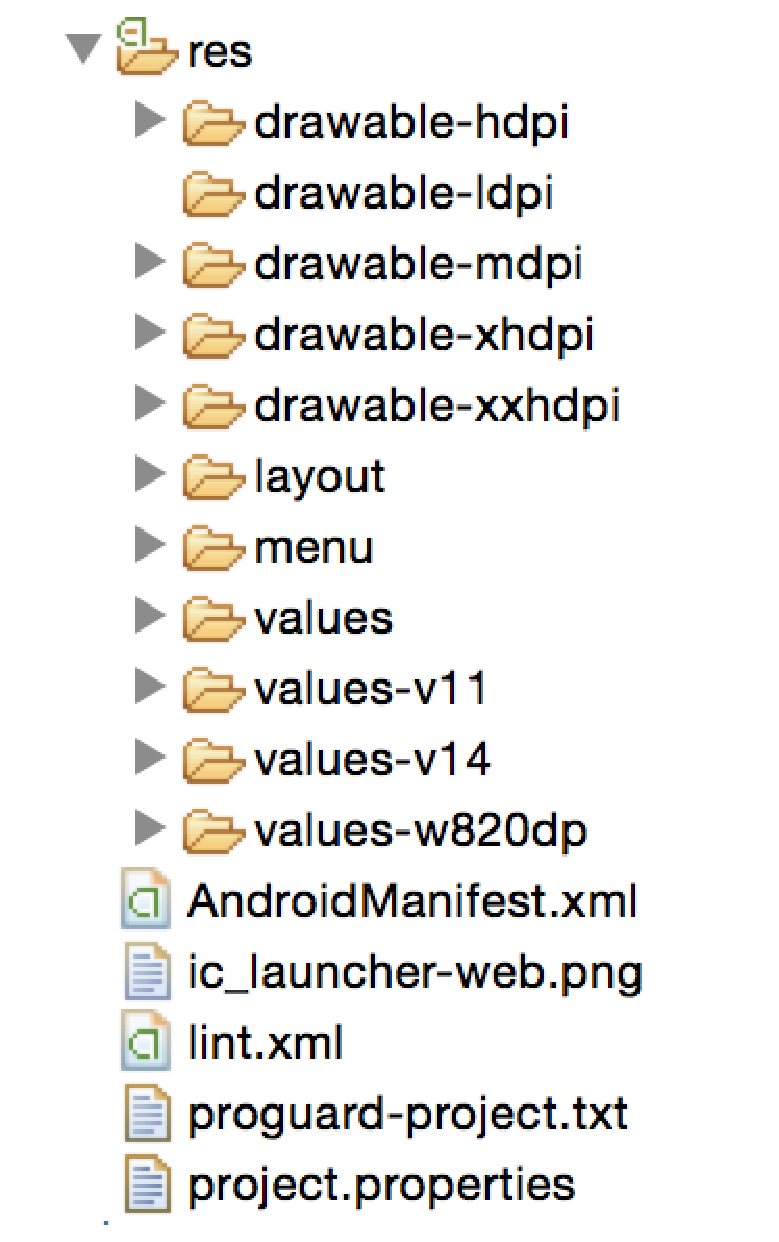
\includegraphics[ scale = 0.2]{resource.eps}
\end{center}
\caption{ res ディレクトリの構成}
\label{res}
\end{figure}

\begin{figure}[t]
\begin{center}
\graphicspath{{./epsfiles/}}
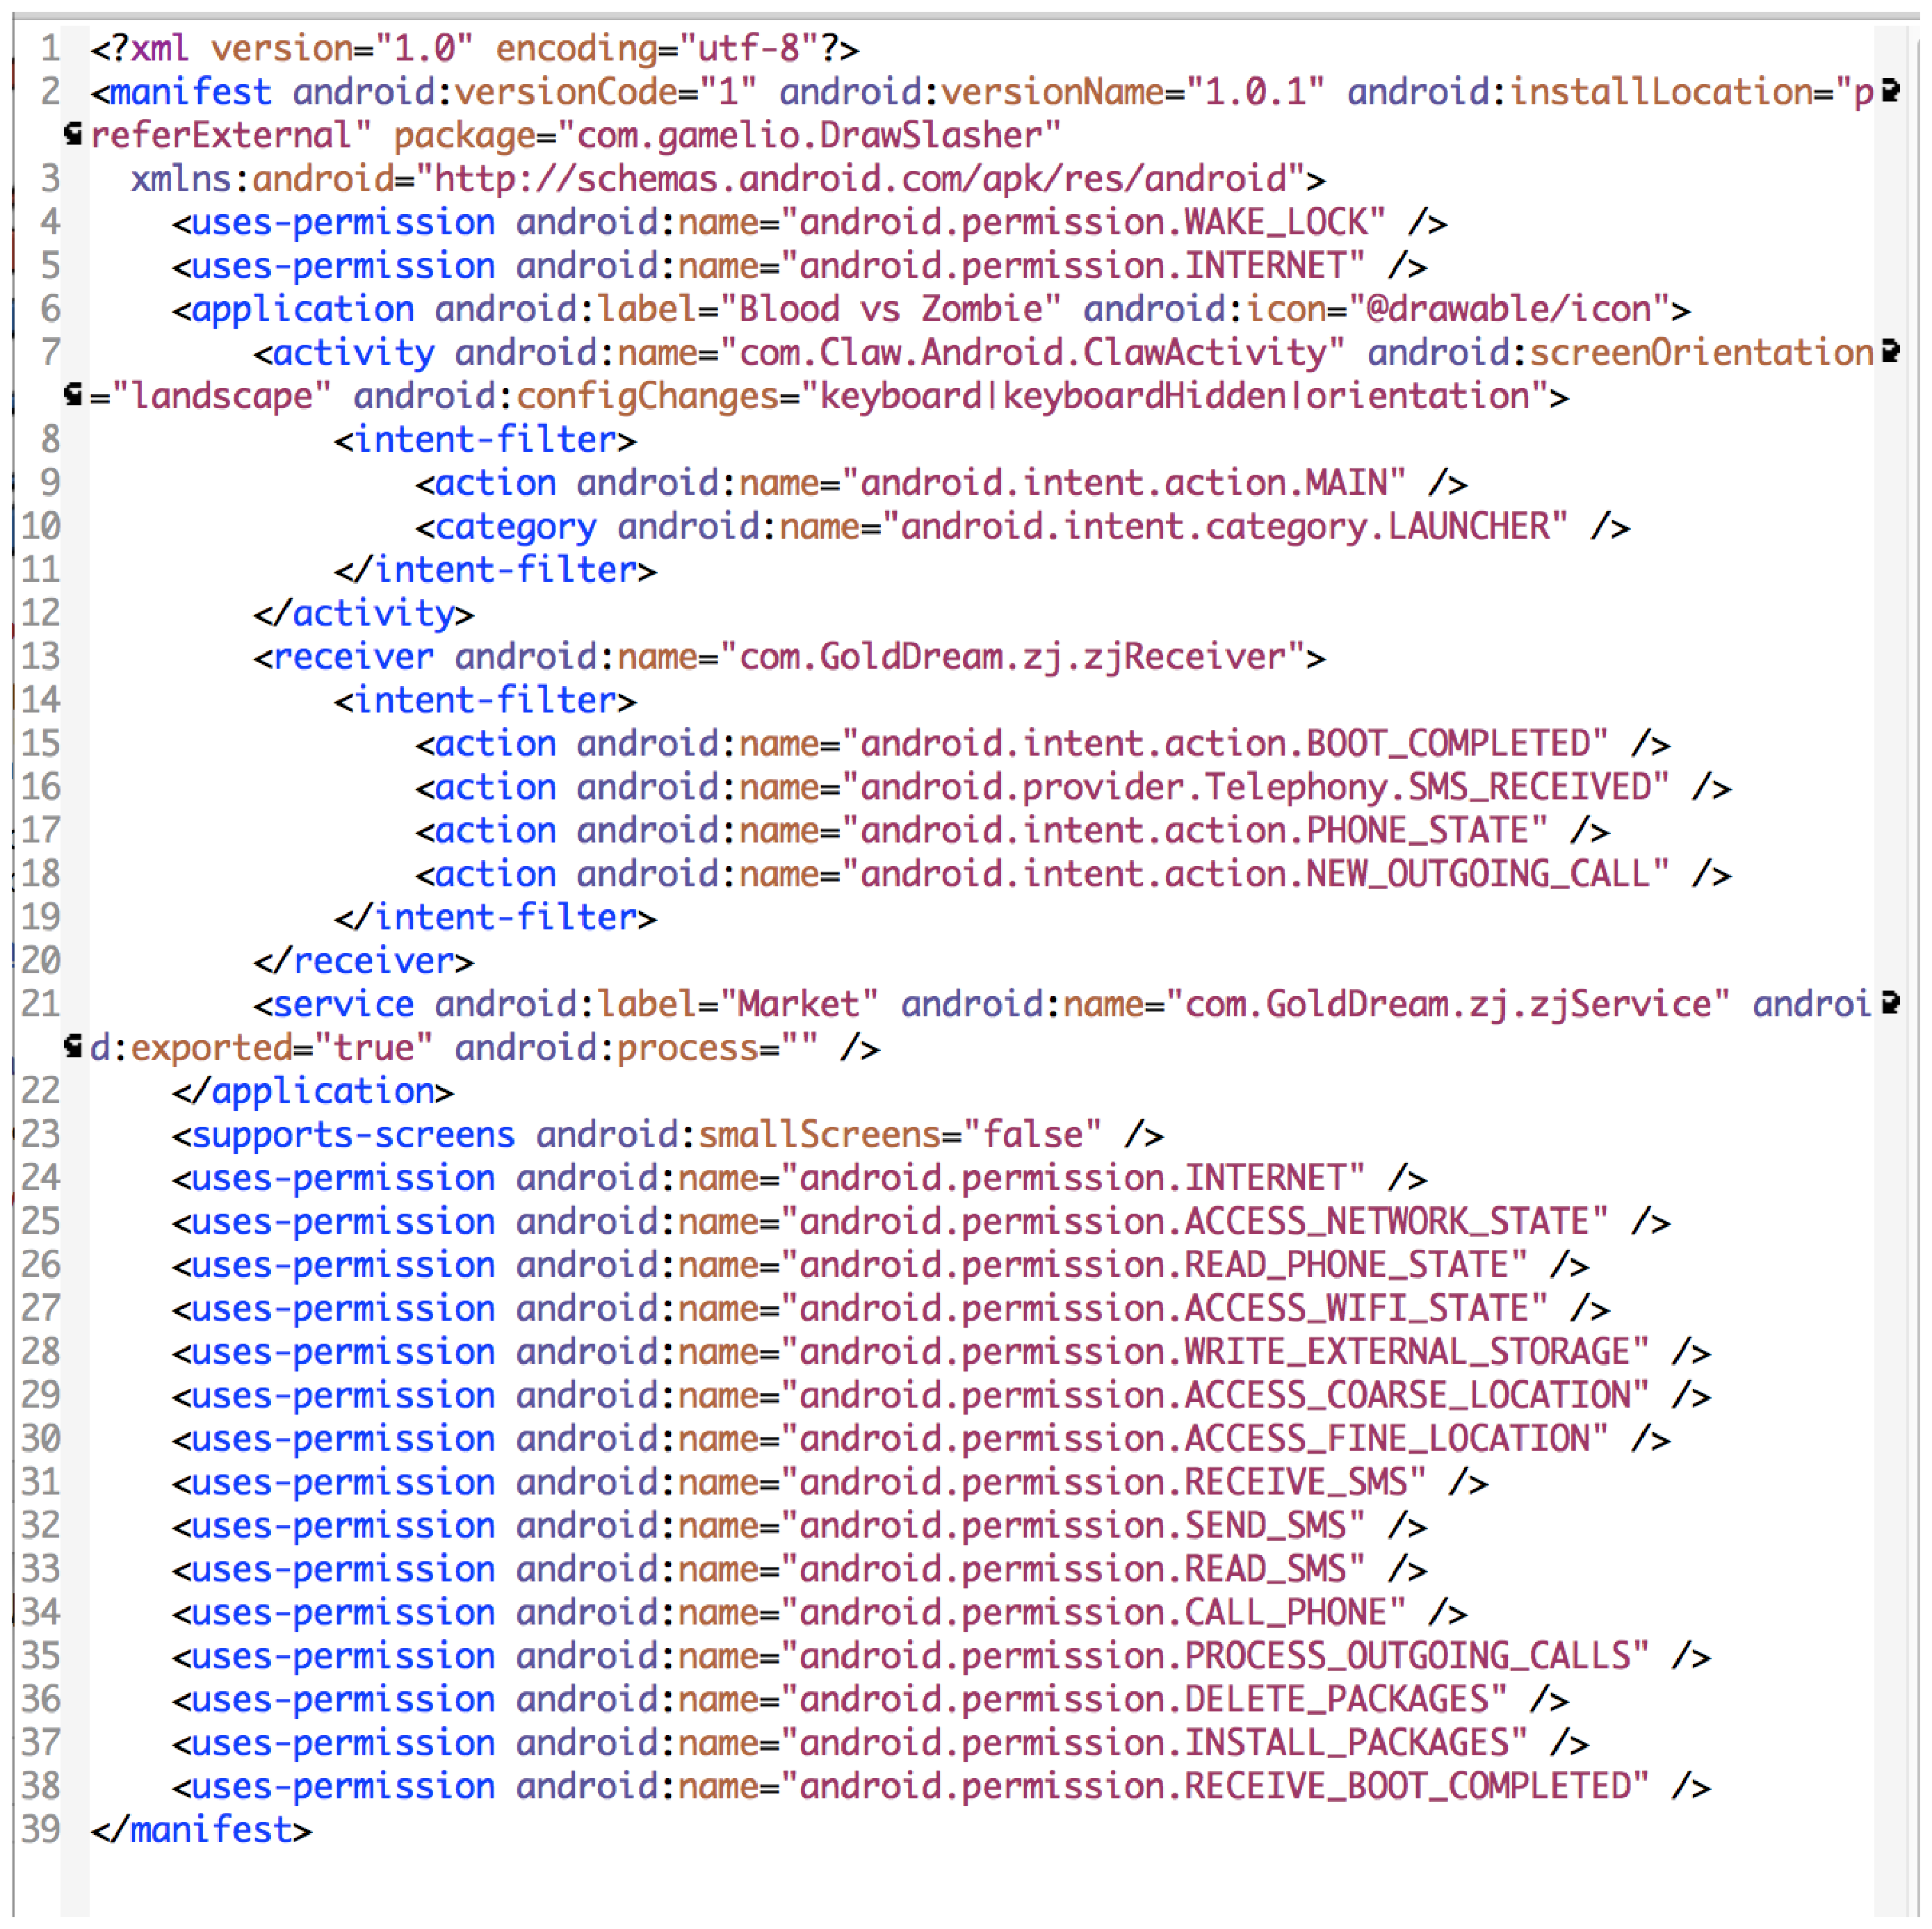
\includegraphics[scale=0.25]{manifest2.eps}
\end{center}
\caption{AndroidManifest.xml の例}
\label{manif}
\end{figure}

